\documentclass[letterpaper, 10 pt, conference]{ieeeconf}

\IEEEoverridecommandlockouts % Needed for the \thanks command

% Needed to meet printer requirements.
\overrideIEEEmargins

%\usepackage{cite}
\usepackage{amsmath}
\usepackage{subcaption}
\usepackage{color} % make comments appear in color.
\usepackage{colortbl}

% Moar spacing for editing.
\linespread{1}

% Color for the table.
\definecolor{Gray}{gray}{0.85}

\usepackage[pdftex]{graphicx}
% declare the path(s) where your graphic files are
\graphicspath{{../MATLAB/LKT/results/} {./figures/}}
% and their extensions so you won't have to specify these with
% every instance of \includegraphics
\DeclareGraphicsExtensions{.pdf,.jpeg,.png}

% Try to make the 'c#' symbol...
\newcommand{\Csharp}{%
  {\settoheight{\dimen0}{C}C\kern-.05em \resizebox{!}{\dimen0}{\raisebox{\depth}{\#}}}}
  
% Argmin and argmax operators.
\DeclareMathOperator*{\argmax}{arg\,max}
\DeclareMathOperator*{\argmin}{arg\,min}

% Comments.
\newcommand{\comment}[1]{{\color{red}[#1]}}
%\newcommand{\comment}[1]{} %NOP

% Formatted subreference.
\newcommand{\Subref}[1]{(\subref{#1})}

% *** SUBFIGURE PACKAGES ***
%\usepackage[tight,footnotesize]{subfigure}
% subfigure.sty was written by Steven Douglas Cochran. This package makes it
% easy to put subfigures in your figures. e.g., "Figure 1a and 1b". For IEEE
% work, it is a good idea to load it with the tight package option to reduce
% the amount of white space around the subfigures.

%\usepackage[caption=false]{caption}
%\usepackage[font=footnotesize]{subfig}
% subfig.sty, also written by Steven Douglas Cochran, is the modern
% replacement for subfigure.sty. However, subfig.sty requires and
% automatically loads Axel Sommerfeldt's caption.sty which will override
% IEEEtran.cls handling of captions and this will result in nonIEEE style
% figure/table captions. To prevent this problem, be sure and preload
% caption.sty with its "caption=false" package option. This is will preserve
% IEEEtran.cls handing of captions. Version 1.3 (2005/06/28) and later 
% (recommended due to many improvements over 1.2) of subfig.sty supports
% the caption=false option directly:
%\usepackage[caption=false,font=footnotesize]{subfig}

% *** PDF, URL AND HYPERLINK PACKAGES ***
%
\usepackage{url}
% url.sty was written by Donald Arseneau. It provides better support for
% handling and breaking URLs. url.sty is already installed on most LaTeX
% systems.



% paper title
% can use linebreaks \\ within to get better formatting as desired
\title{\LARGE \bf Visual Odometry In Inspection Environments}

% author names and affiliations
% use a multiple column layout for up to three different
% affiliations
\author{Priyanka Deo and Howie Choset%
\thanks{Robotics Institute,
Carnegie Mellon University,
Pittsburgh, PA 15213, USA
{\tt\small $\lbrace$ pdeo, choset $\rbrace$@andrew.cmu.edu}}%
}

\begin{document}

\maketitle
\thispagestyle{empty}
\pagestyle{empty}


\begin{abstract}

Inspection robots are valuable tools for surveillance and reconnaissance due to their ability to perform tasks in environments that humans and standard robotic platforms cannot access. In this work, we focus on inspection tasks that take place in confined spaces. In particular, we address current issues with robust localization for a variety of platforms in different confined environments. To accomplish this, we present a framework that enhances Lucas-Kanade tracking by incorporating a salient object tracker. The standard Lucas-Kanade algorithm is used to provide initial motion estimates of the robot's local frame, but has difficulty with large changes in illumination caused by the robot carrying its own light source. Salient environmental features are detected using a Hough Transform and subsequently tracked using a Kalman Filtering approach, but fails if salient features are unavailable or difficult to detect due to environmental conditions. We show that by combining these two approaches, we are able to leverage the individual benefits of each approach to compensate for the weaknesses of the other providing overall enhanced localization. We demonstrate the robustness of our framework by implementing it on and providing results for three separate platforms: a pipe inspection robot, a snake robot traversing the interior of a pipe, and a small treaded \emph{crawler} robot deployed in the interior of a wing box.

\end{abstract}


\section{Introduction}

Inspections are essential to detect problems and maintain structures that degrade over time. However, these inspections must often be conducted in confined spaces that are inaccessible to humans. As a result, robots are attractive platforms to navigate narrow spaces and take video footage of the interior. Accurate localization is important for inspection robots to determine the position of defects found and to navigate to inspect particular locations. For example, localization of defects in pipe inspections helps determine where a pipe needs to be replaced. Similarly, in airplane wing inspections, the robot must navigate the wing to check if components are correctly assembled. 

While inspection robots can be customized for the inspection task at hand, there are common localization challenges faced by all robots in confined spaces, regardless of the platform or task. We are thus interested in localization algorithms that are general enough to be implemented on and effectively used for  a large variety of platforms with minimal tuning or other operator intensive intervention. We propose to use visual odometry to estimate the pose of the robot and combine two standard approaches to get a more robust odometry estimate.

%While inspection robots can be customized for the inspection task at hand, there are common localization challenges faced by all robots in confined spaces, regardless of the platform or task. We are thus interested in localization algorithms that are general enough to be implemented on and effectively used for  a large variety of platforms with minimal tuning or other operator intensive intervention. We propose to combine an approach that is suitable for textured environments with approach that can handle illumination changes to get a more robust odometry estimate.

\begin{figure}[tb]
	\centering
	\begin{subfigure}{.45\columnwidth}
		  \centering
		  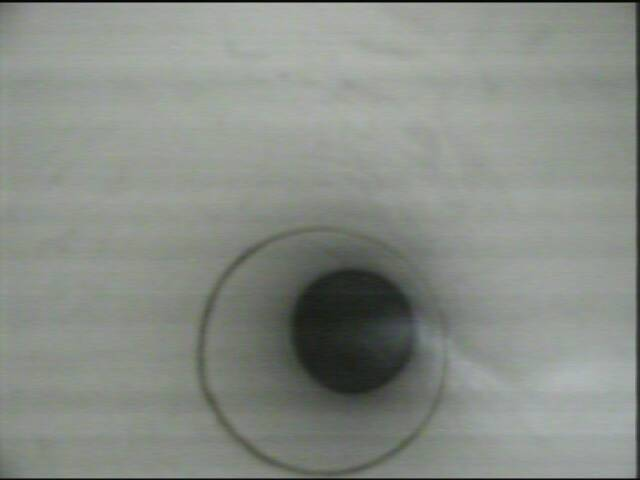
\includegraphics[width=\columnwidth]{pipe_image.png}
		  \subcaption{}
		  \label{example_image:snake}
	\end{subfigure}
	\begin{subfigure}{.45\columnwidth}
		  \centering
		  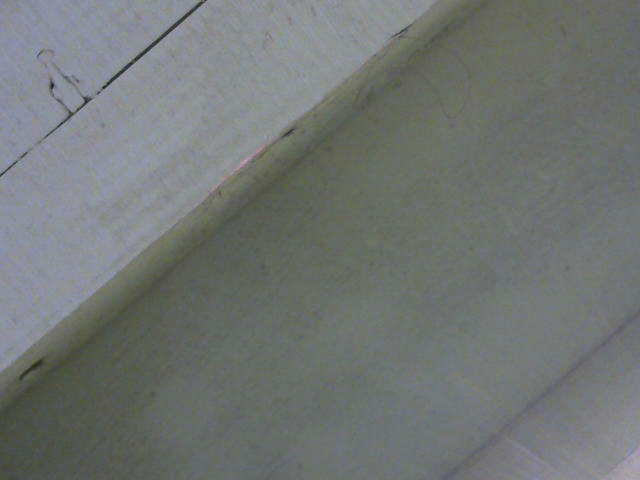
\includegraphics[width=\columnwidth]{wingbay_image.png}
		  \subcaption{}
		  \label{example_image:crawler}
	\end{subfigure}
	\caption{Example images from video taken by the snake robot in a pipe \Subref{example_image:snake} and crawler robot in a mock airplane wing \Subref{example_image:crawler}.}
    \label{example_image}
\end{figure}

\begin{figure}[tb]
	\centering
	\begin{subfigure}{.45\columnwidth}
		  \centering
		  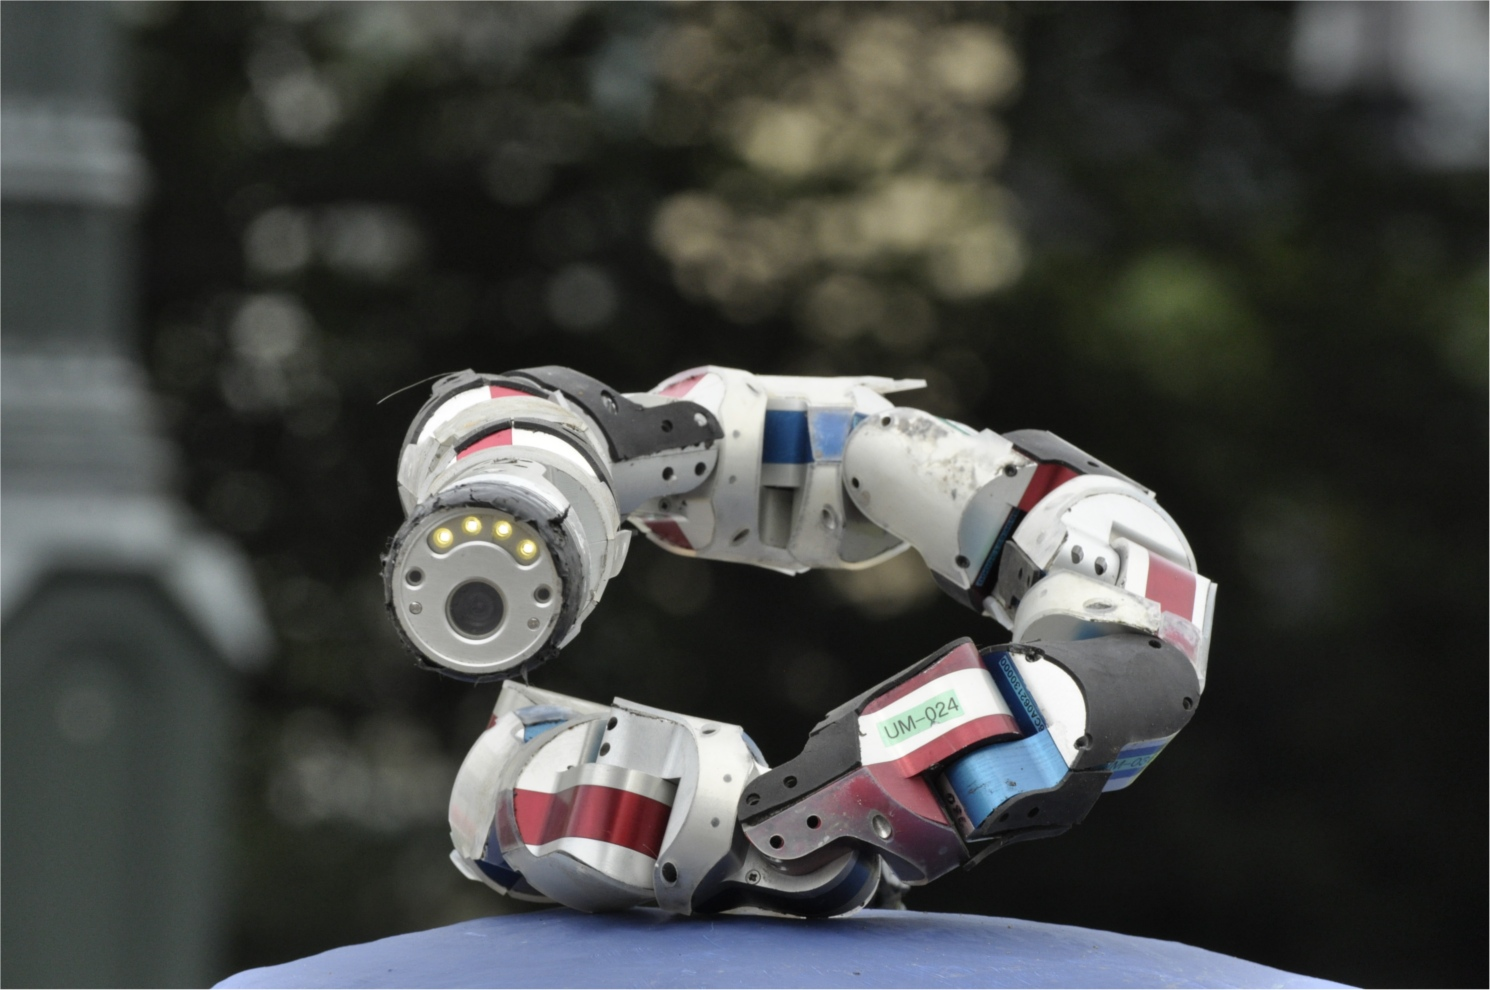
\includegraphics[width=\columnwidth]{snake_image.jpg}
		  \subcaption{}
		  \label{robots:snake}
	\end{subfigure}
	\begin{subfigure}{.45\columnwidth}
		  \centering
		  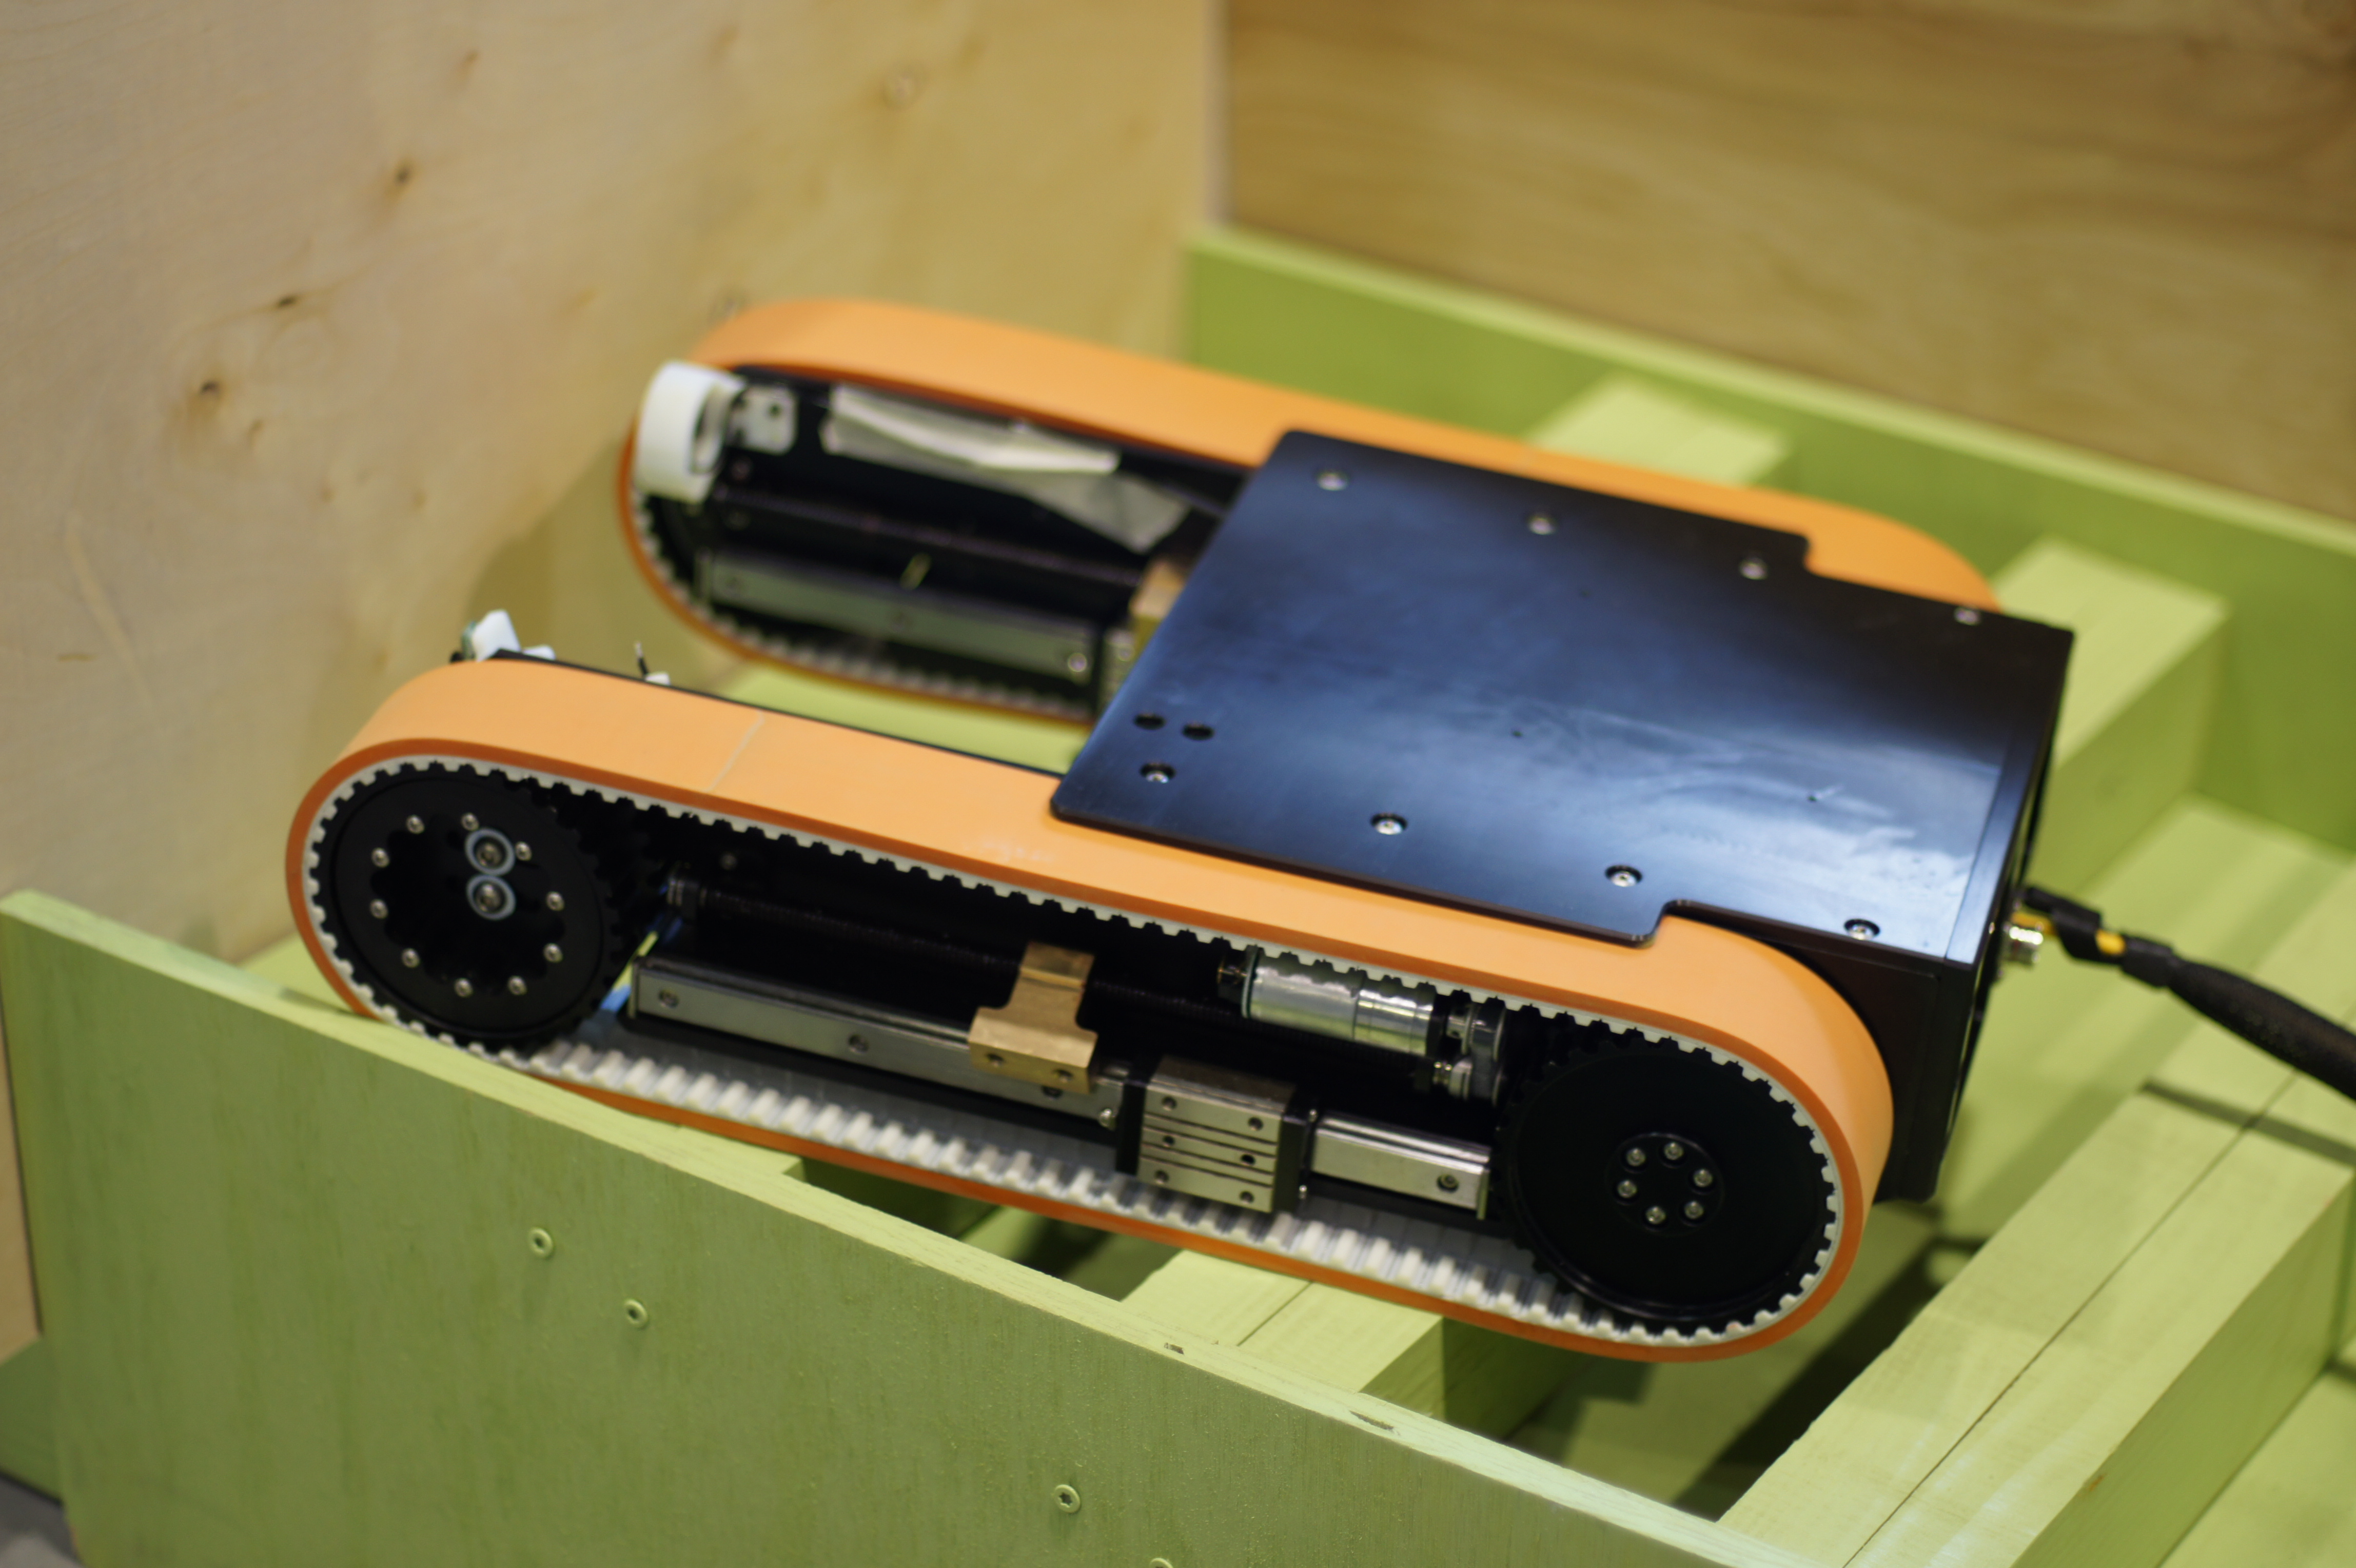
\includegraphics[width=\columnwidth]{crawler_image.jpg}
		  \subcaption{}
		  \label{robots:crawler}
	\end{subfigure}
	\caption{Photographs of the Carnegie Mellon University Biorobotics Lab's \Subref{robots:snake} Unified Modular Snake Robot \Subref{robots:crawler} and Crawler Robot.}
    \label{robots}
\end{figure}

Common approaches for localization in confined spaces include measuring the robot's tether and dead reckoning. Measuring the tether estimates position given that the deployment environment is known to be linear a priori. For localization in more varied environments, dead reckoning can be used to process sensor information to estimate the robot's velocity and, via integration, the robot's position. In many circumstances, dead reckoning produces inaccurate localization results because slip due to the environmental conditions or complexity of the task is not accounted for in primarily first-order dead reckoning approaches. 

%Might want to motivate what feature based and direct approaches are. Cite people? Also you probably want to be citing someone for saying that feature association fails. Talk to Dey about whom to cit otherwise include a figure.

Visual odometry is an alternative to localization that addresses the issues faced in both measuring tether payout and standard odometry. Visual odometry algorithms can be classified as feature-based approaches or direct approaches. 

Feature-based approaches recover the motion of the camera by finding and matching features, usually points of interest, in successive frames and using the correspondences to estimate motion. Feature-based approaches work well in visually rich environments containing many unique trackable features. In inspection environments that are textured, points of interest in the image are self-similar, making stable feature association difficult. 

Instead, direct approaches estimate the motion of the camera directly from the intensity values in the image. The gradient of the intensity is used in an optimization to find the correspondence between two images. For textured environments, direct approaches perform well by using intensity information over the entire image, instead of matching sparse features. However, direct approaches assume differences in pixel intensities are caused by motion and have difficulty with large changes in illumination present in inspection footage.

Visual odometry is challenging in inspection environments that are slightly textured components and are broken up by large edge gradients (see Figure \ref{example_image}). Since the environments considered are enclosed, large changes in illumination occur when a robot with an integrated light source traverses an otherwise unlit environment. Correlating image frames becomes difficult when there are limited features, and large changes in illumination vary the appearances of those features. 

In order to address the challenges of visual odometry in inspection environments, we combine a direct approach to leverage motion information across the entire image with a feature based approach to maintain illumination and drift invariance. Thus, we present a framework for enhancing Lucas-Kanade by incorporating a salient object tracker. We demonstrate the generality and robustness of the approach for robots with different methods of locomotion operating in different environments.

%We present a framework for enhancing Lucas-Kanade tracking by incorporating a salient object tracker, and show improvement over Lucas-Kanade for multiple experimental platforms. We combine a direct approach to leverage motion information across the entire image with a feature based approach to maintain illumination and drift invariance. We demonstrate the generality and robustness of the approach for multiple robots with different methods of locomotion operating in different environments.

We test our approach on a dataset of videos from pipe inspection robots published by sewer inspection companies on YouTube. We also perform experiments using a snake robot (Fig. \ref{robots:snake}) crawling through a pipe, and a crawler robot (Fig. \ref{robots:crawler}) driving in a mock airplane wing. The test platforms are described further in Section \ref{section:Experimental Platforms}.


\section{Approach}

%Figure \ref{approach} shows an overview of the integration of a salient object tracker with the Lucas-Kanade pipeline. Lucas-Kanade produces an estimate of motion by comparing a new image frame with a previously localized frame. The salient object tracker uses a Hough Transform to detect an object in the new image frame that is tracked via a Kalman Filter, producing another estimate of motion. The robot's motion is estimated as the weighted average of the estimations produced independently by Lucas-Kanade and the object tracker. The final motion estimate is integrated to determine the state of the robot relative to its initial position.


\comment{Fix this introductory sentence.} Since the inspection environments considered are textured with few features, direct approaches are more appropriate. Lucas-Kanade \cite{Lucas81, lucaskanade} is used to find the relative motion between image frames in the footage taken by the robot. The direct approach can be combined with a feature-based approach to gain illumination invariance. Structural features of the environment are detected using a Hough transform \cite{Hough59, Ballard81} and tracked using a Kalman filter \cite{Kalman82}. Estimates of pose from the direct approach and the feature-based approach are combined using a high-level Kalman filter observing the robot's motion. The Kalman filter helps smooth noise and detect measurement outliers and provides a framework for combining multiple pose estimates. Since the motion measurements are in the image frame, the scale between the image and the environment must be extracted. The size of the tracked objects in the image is compared to the known size of the object in the environment. These comparisons give the scale between the robot's pose estimated by the visual odometry algorithms and the robot's pose in the environment. Figure \ref{approach} provides an overview of the integration of a salient object tracker with Lucas-Kanade.


%\begin{itemize}
%\item Since direct approaches work for textured environments with few features, it is more appropriate for inspection evironments. We can use a direct approach to get an estimate of motion that is illumination invariant. We specifically use Lucas-Kanade as our direct approach.
%
%\item We want to combine this with a feature-based approach to get illumination invariance. We create a salient object tracker, by combining a Hough transform to detect objects with a Kalman filter to track them.
%
%\item We propose to combine both approaches using a Kalman filter. Kalman filter helps smooth out noise. We have a framework to add other estimates of motion easily. We can detect outliers using the covariance.
%
%\item This gives us a final estimate of motion. We can integrate the motions to get a position.
%
%\item Since the measurements of the visual odometry algorithms are in the image frame, we need to extract scale between the image and the environment. We do this in the scale extraction process, by comparing tracked objects and their known size in the environment.
%
%\item This gives us an estimate of pose in the real world.
%\end{itemize}


\begin{figure}[tb]
	\centering
	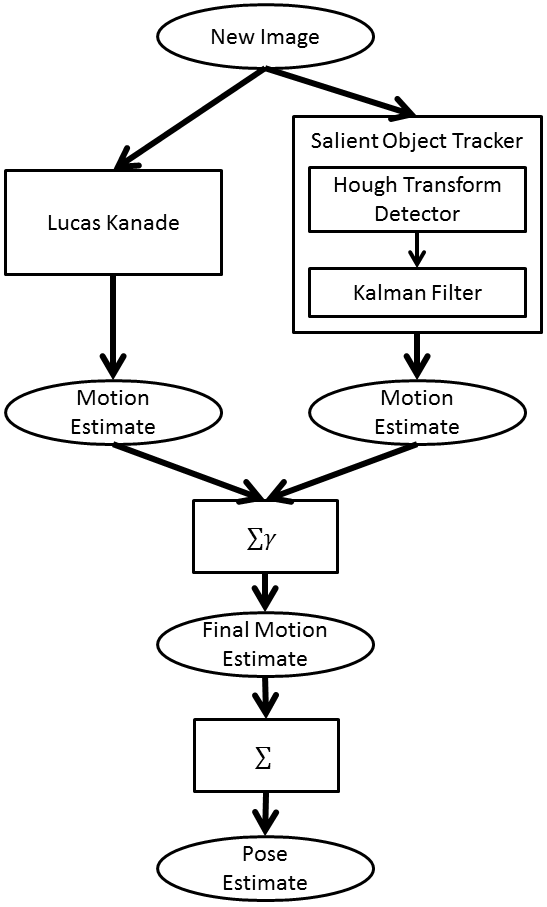
\includegraphics[height=200px]{approach_overview.png}
	\caption{Visual odometry pipeline with feature tracking.}
    \label{approach}
\end{figure}

\subsection{Lucas-Kanade}

\comment{You should really motivate why Lucas-Kanade here.}

Direct approaches compare the pixel intensities of two images to determine the correspondence between them. One image is transformed to match the other image, which serves as a template. Lucas-Kanade finds the transform that minimizes the total error in pixel intensities between the transformed image and the template image. The transform is described using a set of parameters that are optimized by Lucas-Kanade. The parameters are refined using the gradient of the template image to minimize the error in pixel intensities. 

For all pixels $\psi$, the error between the transformed image $I$ and the template image $T$ is computed. Lucas-Kanade finds the parameters $p$ of the transform $W$ that minimizes the sum of squared error in intensity, 

\begin{equation} \label{eq:lkt_min}
    \argmin_p \sum_{\psi} [I(W(\psi, p)) - T(\psi)]^2.
\end{equation}

Lucas-Kanade is used to find the relative motion between image frames in the inspection footage taken by the robot. Every image in the video is localized with respect to an earlier frame that has already been localized. Since the robot has little motion between consecutive frames, image frames are compared to nearby frames in the video to ensure sufficient visual similarity between the images to accurately relate them.

For our applications, since the robot has limited motion in the inspection environments, the image transform is constrained to rotations, translations, and scale. Motions of the robot in the image plane ($\Delta x$, $\Delta y$, and $\Delta \theta$) correspond directly to motions of the image. Motion of the robot into the image plane ($\Delta z$) manifests as a change in image scale, proportional to the focal length $f$ of the camera. To simplify further equations, the robot's motion into the image plane can be written using the change in image scale $\alpha$,

\begin{equation} \label{eq:z_motion_conversion}
	\alpha = 1 - \frac{\Delta z}{f}.
\end{equation}

When the robot takes a new image, the transform between the new image and the template image described in terms of the robot's motion will have the form,

\begin{equation*}
W(\Delta x, \Delta y, \Delta \theta, \alpha) = \begin{bmatrix} \frac{\cos(\Delta \theta)}{\alpha} & -\frac{\sin(\Delta \theta)}{\alpha} & \frac{\Delta x}{\alpha} \\ \frac{\sin(\Delta \theta)}{\alpha} & \frac{\cos(\Delta \theta)}{\alpha} & \frac{\Delta y}{\alpha} \\ 0 & 0 & 1 \end{bmatrix}.
\end{equation*}

\comment{Integrate paragraphs better.} Since we are looking at video from a robot which has smooth movements, image frames that are temporally close in the video must also be \comment{spatially close in the environment isnt quite right.} spatially close in the environment. 
\comment{Casual.} Since image frames must have enough visual similarity to be accurately correlated, there must be small spatial motion between the images. Since there is small spatial motion, there is small rotation. We can linearize around a small rotation to give an approximation of the transform with a simpler representation.


%Since the image frames being compared are temporally close, they must also be spatially close. Linearizing around small rotations gives an approximation to the transform,

\begin{equation*}
W(\Delta x, \Delta y, \Delta \theta, \alpha) = \begin{bmatrix} \frac{1}{\alpha} & -\frac{\Delta \theta}{\alpha} & \frac{\Delta x}{\alpha} \\ \frac{\Delta \theta}{\alpha} & \frac{1}{\alpha} & \frac{\Delta y}{\alpha} \\ 0 & 0 & 1 \end{bmatrix}.
\end{equation*}

The set of parameters optimized during the Lucas-Kanade minimization can be \comment{extracted is not the right word.} extracted from the robot's motion. 
\comment{Casual. Fix.} We can then write the transform in terms of these parameters,

%For convenience, during the Lucas-Kanade minimization, the transform can be rewritten in terms of a set of independent parameters,

\begin{eqnarray}
\begin{split} \label{eq:warp_param_conversion}
p_1 &=& \frac{\Delta x}{\alpha}\\
p_2 &=& \frac{\Delta y}{\alpha}\\
p_3 &=& \frac{\Delta \theta}{\alpha}\\
p_4 &=& \frac{1}{\alpha} - 1\\
\end{split}
\\ \label{eq:param_warp}
W(p) = \begin{bmatrix} 1+p_4 & -p_3 & p_1 \\ p_3 & 1+p_4 & p_2 \\ 0 & 0 & 1 \end{bmatrix}.
\end{eqnarray}

We solve the resulting minimization problem \eqref{eq:lkt_min} with the parameterized transform \eqref{eq:param_warp} using the method of Lucas and Kanade \cite{Lucas81, lucaskanade}, which provides an estimate of the relative motion between the template and the current image frame. The robot's motion can be recovered from the transform parameters using Equation \eqref{eq:z_motion_conversion} and Equation \eqref{eq:warp_param_conversion}.

Since motion is determined relative to the template image, errors in the localization compound when the template is updated. Therefore, instead of updating the template every frame, the same template is used to localize several consecutive images, reducing drift.
\comment{integrate this better with the paragraph.} However, as the robot moves the new images move further from the template image, breaking the assumption of spatially closeness to the template, making the linearization worse. 
\comment{Integrate this better with the paragraph.} In order to ensure that image comparisons are temporally and spatially close, the template is updated to the last localized image frame when the robot has traveled beyond some threshold distance and the field of view has changed.
\comment{How do you choose this threshold?  What happens if the field of view hasn’t really changed.  Exactly when do you decide the linearization fails…justify your decisions.} This threshold is set by the user based on the environment, so that images have little motion up to the point of the thresholded distance. If objects are close to the camera, this number must be smaller than if the objects were further away. If the field of view hasn't changed then we update more than necessary. If the field of view has changed, the linearization will be poor and Lucas-Kanade will have worse performance.

\subsection{Salient Object Tracking}

In the inspection environments considered, structural elements, such as pipe joints or airplane ribs, can be tracked to improve motion estimates and illumination invariance. These repeating structural elements are salient objects distinguishable from the textured environment, making them ideal for tracking. Since these salient objects are geometric shapes, the objects can be detected by determining which points in the image form the boundary of a given shape. Points on the boundary of the shape are detected using an edge detection algorithm. The Hough transform is used to determine which points correspond to the same shape. The location of the object is then tracked using a Kalman filter. The motion of the robot is inferred from the motion of the object.

%In an inspection environment, large features, such as pipe joints or airplane ribs, can be tracked to improve motion estimates. These salient objects can be detected in an image using a Hough Transform.

In our approach, we track one salient object, such as a pipe joint or an edge of the airplane rib, in each frame of the inspection footage taken by the robot. If multiple objects are present, the object with the stronger Hough transform score is used to initialize the tracker. The Hough transform parameters define the location of the object and can be used as the object's state when tracking. Since the robot has little motion between consecutive frames of the video, the state of the object is assumed to be close to the previous state.

%In our approach, we track one salient object, such as a pipe joint or an edge of the airplane rib. The state of the object is represented using the parameterized space defined by the Hough transform.  Since the robots exhibit smooth motion, the current state of the object should be close to the previous state. The current state is estimated to be the parameters of an object found using the Hough transform that has both a high Hough transform score and is close to the previous state.

Salient objects are detected by finding several points that form the boundary of a geometric shape. Whether a set of points form a given shape cannot be clearly determined by looking at x-y image locations of the points. Instead, the Hough transform is used to transform points from the x-y space to a parameterized space, where points that correspond to the same shape have one common parameterization. For example, a straight line is parameterized by the angle and length of the normal vector to that line from a reference point, usually a corner of the image. While each point on the line corresponds to multiple potential lines passing through that point, all points share one correspondence in common.

%The Hough transform defines a parameterized space based on the shape of the object being identified. For example, a straight line is parameterized by an angle $\theta$ and a length $\rho$, and a circle is parameterized by a center $(a, b)$ and a radius $r$.

For each point detected using an edge detection algorithm, the Hough transform determines a set of shapes that the point corresponds to and explains. A shape that can be explained by multiple points has more evidence for being a true detection. The Hough transform finds shapes that are explained by a large number of points and are likely to be present in the image. The Matlab implementation of Hough transforms also returns a score that measures the relative strengths of the detected objects.

%Points on edges in the image are first identified using an edge detection algorithm. For each of the identified points, the Hough transform determines a set of objects that explain the local edge gradients. The point casts a vote for each of these objects in the parameterized space. The most likely objects are extracted by finding regions in the parameterized space that have a large number of votes. The Matlab implementation of Hough transforms also returns a score that measures the relative strengths of the detected objects.

The Hough transform finds multiple geometric shapes in an image that may correspond to the object being tracked. To determine whether any of the candidate object detections are good estimates of the tracked object, a similarity score is defined to measure the quality of the detection. To compute the score, each candidate object is described by a feature descriptor that is a vector containing the Hough transform score and the difference in Hough parameters between the candidate and the previous state. The feature descriptor contains information about the quality of the Hough detection and the similarity to the previous state. The similarity score is computed using the feature descriptor $\textbf{F}$ and a set of tuned feature weights $w$ for a given type of tracker. The state of the object is estimated as the detection in the set of candidate object detections $O$ with the best score,

%To estimate the current state from the set of candidate objects $O$ that are found using the Hough transform, we define a feature descriptor $\textbf{F}$ and a similarity score based on the feature descriptor that measures the quality of a detection. The feature descriptor is a vector containing the Hough Transform score and the difference between the Hough parameters of the candidate object and the previous state. The similarity score can be computed using a set of tuned feature weights $w$ for a given type of tracker,

\begin{equation} \label{eq:similarity_score}
	s_{k} = \argmax_{o_i \in O} w^T \textbf{F}(o_i).
\end{equation}

Tracking the object using only the similarity score to estimate the state is noisy and prone to outliers. Often the estimated object will display erratic movement that is not consistent with motion of the physical system. Tracking is improved by using a Kalman Filter with a first-order model of the state $s$ of the object, with process noise $\nu \in N(0, \mu_1)$ and measurement noise $\omega \in N(0, \mu_2)$,

\begin{eqnarray*}
s = \begin{bmatrix} P \\ \dot{P} \end{bmatrix} \\
s_{k+1} = \begin{bmatrix} I & dt * I \\ 0 & I \end{bmatrix} s_{k} + \nu \\
y_k = \begin{bmatrix} I & 0 \end{bmatrix} s_k + \omega.
\end{eqnarray*}

A salient object is tracked until it moves out of the image frame and out of the field of view. The search for a new object is biased towards the last state of the previously tracked object. For example, circles are reinitialized with similar centers, since new objects are likely to be in the same location but closer or further away. Similarly, lines are reinitialized with similar orientations, since new objects are likely to be in a different location but have a similar orientation. New objects are initialized by finding a candidate object detection with a high Hough transform score that has parameters similar to the last state of the previously tracked object. We can again use the similarity score \eqref{eq:similarity_score} to choose between candidate object detections, and can threshold the score to filter bad initializations. 

%A salient object is tracked until it moves out of the image frame and out of the field of view, at which point a new object is initialized. For the snake robot and pipe inspection videos, the search is biased towards small circles near the center of the previously tracked object. For the crawler robot, the search is biased towards lines with the same orientation as the previously tracked object.

The motion of the robot is inferred using the change in state of the salient object. Changes in the location of the object in the x-y plane of the image correspond to planar motions of the robot  ($\Delta x$, $\Delta y$, and $\Delta \theta$). For circular objects, orientation cannot be estimated due to symmetry. Motion of the robot into the image plane ($\Delta z$) corresponds to changes in the size of the object in the image. When tracking lines, motion into the image plane cannot be estimated because the length of the line is not a good estimate of size.

%The motion of the robot can be inferred using the change in state of the salient object. Motions of the object in the x-y plane of the image correspond to planar motions of the robot  ($\Delta x$, $\Delta y$, and $\Delta \theta$). For circular objects, orientation cannot be estimated due to symmetry. Changes in the size of the object correspond to motions of the robot into the image plane ($\Delta z$). For linear objects, motion into this plane cannot be estimated because the length of the line is not a good estimate of size.

%\subsection{Combining Estimates}
%
%\subsection{Extracting Scale}
%
%Both Lucas-Kanade and the salient object tracker measure the robot's motion using image pixels. In order extract physical distances, scale between image pixels and physical objects must be determined.
%
%For the pipe inspection videos and the snake robot, the scale is computed through the known radius of the pipe. The Youtube videos are annotated with the radius found by physically measuring the pipe. For the snake robot, the pipe radius was physically measured, but could also be estimated using the robot's joint angles \cite{Enner2013}.
%
%When the salient object tracker detects a pipe joint, the radius of the joint in the image is measured. Scale is estimated as the ratio between the known radius of the pipe and the measured radius of the tracked joint. Estimates of the robot's distance to the joint are calculated using the scale and the camera's focal length. For situations where the camera cannot be calibrated, as with the Youtube videos, the camera's focal length is estimated to be the same as a Microsoft Kinect because it has a standard published focal length.
%
%For the airplane wing inspection videos, the camera faces the ribbed ceiling of an airplane wing at a constant distance. Since the width of the beams on the ceiling is known, scale is estimated using noisy measurements of the beams in the image with an approach similar to \cite{Lucey14}. Scale is repeatedly refined with new measurements of the beam width until convergence, when a fixed value is used.
%
%Beams are located in an image using a Hough Transform, as described previously, to detect lines in the image. We assume that the two most parallel lines in an image form the boundary of a beam. Instances when the assumption is incorrect are treated as part of noise in the data and are accounted for when finding the best scale factor.
%
%We measure the pixel distance between the two parallel lines to get a noisy estimate of the width of the beam. All measurements of beam width in the image are concatenated into a vector $\textbf{W}$, and are compared to a vector $\textbf{B}$ of the known physical measurements. The scale $\beta$ between pixel measurements and physical units is computed by minimizing the error between the physical beam width and the scaled pixel beam widths,
%
%\begin{equation}
%	\argmin_{\beta} ||\textbf{B} - \beta \textbf{W} ||.
%\end{equation}
%

\section{Experimental Platforms} \label{section:Experimental Platforms}

%We performed experiments on a dataset of pipe inspection videos from Youtube as well as on the snake robot and the crawler robot.
%
%The Youtube dataset consists of four videos \cite{pipevideo2, pipevideo4, pipevideo5, pipevideo6} posted by pipe inspection companies of first-person footage from inspection robots equipped with lighting and a camera as they navigate through a pipe. These videos are annotated with ground truth distance that the robot has traveled as measured via the robot's tether. This data contains videos taken in pipes of varying size, material, and conditions.
%
%The snake robot \cite{Wright2012} consists of a series of identical 1-degree-of-freedom (DOF) joints oriented at $90^{\circ}$ relative to one another and locomotes using cyclic patterns of joint motion. Previous work with the snake robot has used a motion model \cite{Enner2012} to estimate the motion of the robot in straight pipes \cite{Enner2013}. This approach uses the joint angles and kinematics of the snake robot to estimate how much the snake has moved. This is analogous to a integrating the encoders on a wheeled robotic system, and does not account for slip.
%
%The crawler robot is a small treaded robot with a camera facing up and a camera facing towards the rear, built to investigate airplane wings. Localization is provided by tracking a fixed April Tag with the rear-facing camera. Such localization fails if the April Tag is out of the field of view of the camera, or when the robot is far from the tag and pixel errors in tag localization correspond to large errors in distance.

\section{Experiment Results}

%We tested our algorithm on a Youtube dataset of four different pipe inspection videos that were split into a total of five 1-minute segments for ease of processing. This dataset was used to measure accuracy on a several videos with ground truth. Sections where the robot turned its camera away from the downstream direction of the pipe were removed because the joint was not visible. If we had control over the robot, cropping the video would not be necessary because the tracker could be paused until the robot returned to looking downstream. Every frame in this dataset is correlated with an estimate of forward distance traveled measured using the robot's tether. To avoid incorrect accuracy estimates, the dataset is limited to sections of the video where the robot is moving forward or stopped, and the tether estimate reflects the robots motion well.
%
%\begin{table*}[tb] 
%	\centering
%	\footnotesize
%	\setlength{\tabcolsep}{.5em}
%	\caption{Error Statistics on Youtube Dataset}
%	\label{table:youtube_results}
%	\begin{tabular}{c|c|c|c|c|}
%		\hline
%		& Algorithm & Max Error & Mean Error & Standard Deviation of Error\\
%		\hline
%		Pipe Video 1 & LKT & 16.5 & 7.702 & 4.692 \\
%		\rowcolor{Gray}
%		Pipe Video 1 & LKT + Joint Tracking & 3.098 & 1.678 & 0.8218\\
%		Pipe Video 2 & LKT & 12.56 & 5.009 & 4.032\\
%		\rowcolor{Gray}
%		Pipe Video 2 & LKT + Joint Tracking & 2.685 & 1.38 & 0.7038\\
%		Pipe Video 3 & LKT & 0.8046 & 0.6841 & 0.1872 \\
%		\rowcolor{Gray}
%		Pipe Video 3 & LKT + Joint Tracking & 3.19 & 2.128 & 0.4301\\
%		Pipe Video 4 & LKT & 16.69 & 7.747 & 5.138\\
%		\rowcolor{Gray}
%		Pipe Video 4 & LKT + Joint Tracking & 21.09 & 10.33 & 6.834\\
%		Pipe Video 5 & LKT & 16.79 & 8.86 & 5.228 \\
%		\rowcolor{Gray}
%		Pipe Video 5 & LKT + Joint Tracking & 7.024 & 3.441 & 2.073\\
%		\hline
%		\hline
%		Average  & LKT & 10.96 & 5.1311 & 3.3384 \\
%		\rowcolor{Gray}
%		Average & LKT + Joint Tracking & 7.0081 & 3.5471 & 2.0579\\
%		\hline
%	\end{tabular}
%\end{table*}
%
%
%Overall, the salient object tracker improves the Lucas-Kanade position estimates by reducing the average error as shown in Table \ref{table:youtube_results}. On average, incorporating the salient object tracker reduces the maximum error of Lucas-Kanade by $36 \%$ and the mean error by $31 \%$. For videos 3 and 4, the salient object tracker fails when there is not enough light to enhance textures along the pipe wall, making it difficult to detect joints. Repeated failures of the object tracker results in a higher maximum error and higher mean error on these videos.
%
%
%We threshold the average pixel intensity value over the entire video to determine apriori whether a particular pipe video has enough lighting for the salient object tracker to perform well. Videos 1 and 2 had the highest average pixel intensity values and also corresponded to videos where the salient object tracker improves upon the Lucas-Kanade algorithm the most (see Figure \ref{youtube:error_over_time}). These two videos improved the mean error by $76 \%$ on average.
%
%
%\begin{figure}[tb]
%	\centering
%	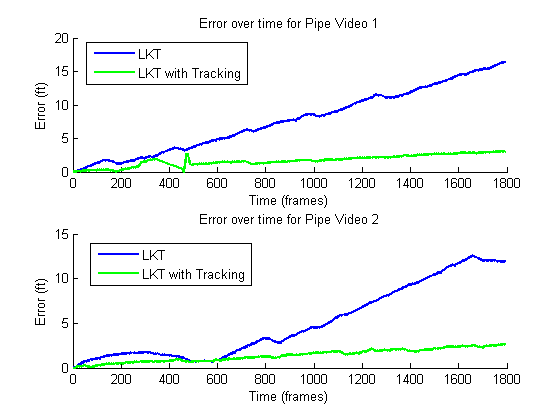
\includegraphics[width=\columnwidth]{youtube_err_v_time.png}
%	\caption{Error between the different algorithms and the groundtruth for the Youtube videos.}
%    \label{youtube:error_over_time}
%\end{figure}
%
%
%We carried out experiments with the snake robot and the crawler robot to compare the performance of Lucas-Kanade with and without salient object tracking. We collected data for two sets of motions with each of these robots.
%
%For the snake robot, the first motion (dashed line in Fig. \ref{snakes:trial8_path}) consisted of unimpeded motion within the pipe, while the second motion (dashed line in Fig. \ref{snakes:trial9_path}) simulated infinite slip when the robot was held in place. The groundtruth was estimated by measuring the amount of tether released at the end of each motion and when the robot was held in place.
%
%The motion model for the snake robot slightly underestimates the actual robot motion when unimpeded (Fig. \ref{snakes:trial8_path}) and fails to adjust for holding the robot in place (Fig. \ref{snakes:trial9_path}), since it has no notion of friction or slip. In contrast, Lucas-Kanade and the salient object tracker are maintian a consistent position estimate when the robot is held in place. Compared to the actual measurement of $0.1714$m for the point when the robot was held in place, the Lucas-Kanade estimate is $0.1831$m, while incorporating the salient object tracker slightly improves the estimate to $0.1823$m. 
%
%Figure \ref{snakes:trial8_error} shows that even though all three estimates drift from the true position of the robot, incorporating the salient object tracker helps improve motion estimates from Lucas-Kanade. In Figure \ref{snakes:trial9_error}, Lucas-Kanade with and without the object tracker both accumulate a large amount of error after frame 600, when the robot's field of view faces the side of the pipe and when joint moves behind the camera. Since the pipe is made of PVC and has little texture and the joint is out of the field of view, both vision based methods have poor estimates of relative motion.
%
%Overall, Lucas-Kanade has a final error estimate of $18.6 \%$ of the distance traveled for the first motion and $45.7 \%$ for the second motion, while Lucas-Kanade with the object tracking has a final error estimate of $2 \%$ of total distance traveled for the first motion and $61.6 \%$ for the second motion. Incorporating the salient object tracker improves estimation for the first motion, but causes more drift for the second motion.
%
%\begin{figure*}[tb]
%	\centering
%	\begin{subfigure}{\columnwidth}
%		  \centering
%		  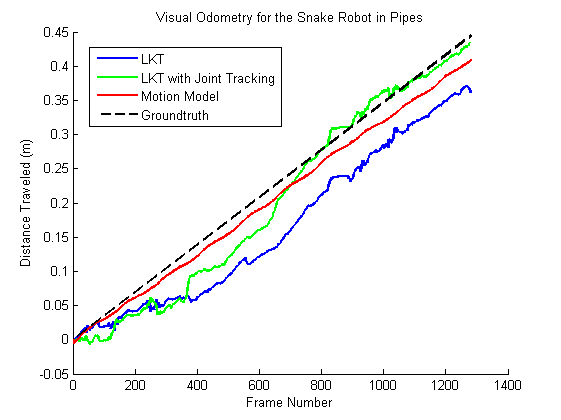
\includegraphics[width=\columnwidth]{trial8_path.png}
%		  \subcaption{Paths produced by different motion estimates when the robot drives continuously within the pipe.}
%		  \label{snakes:trial8_path}
%	\end{subfigure}
%	\begin{subfigure}{\columnwidth}
%		  \centering
%		  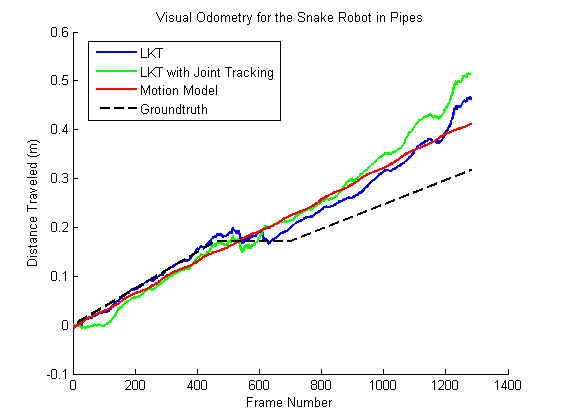
\includegraphics[width=\columnwidth]{trial9_path.png}
%		  \subcaption{Paths produced by different motion estimates when the robot is temporarily held in place while driving within the pipe.}
%		  \label{snakes:trial9_path}
%	\end{subfigure}
%	\caption{Odometry paths generated for multiple motions using the snake robot.}
%    \label{snakes_path}
%\end{figure*}
%
%\begin{figure*}[tb]
%	\centering
%	\begin{subfigure}{\columnwidth}
%		  \centering
%		  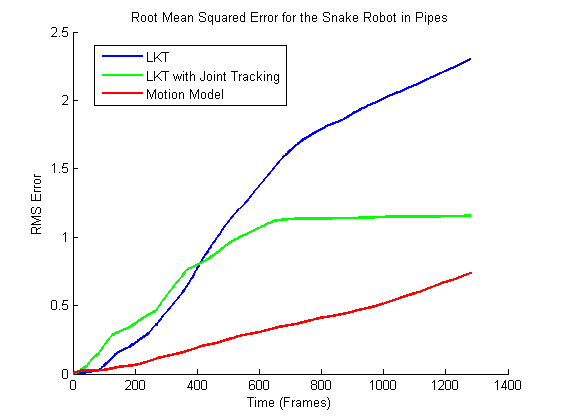
\includegraphics[width=\columnwidth]{trial8_rms.png}
%		  \subcaption{Error between different algorithms for driving the robot continuously within the pipe.}
%		  \label{snakes:trial8_error}
%	\end{subfigure}
%	\begin{subfigure}{\columnwidth}
%		  \centering
%		  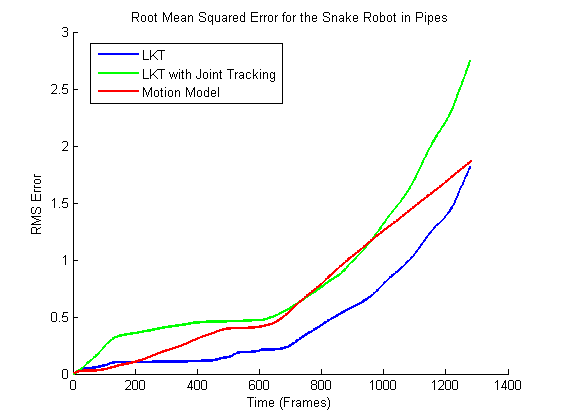
\includegraphics[width=\columnwidth]{trial9_rms.png}
%		  \subcaption{Error between different algorithms for temporarily holding the robot in place while driving within the pipe.}
%		  \label{snakes:trial9_error}
%	\end{subfigure}
%	\caption{Comparison of errors between algorithms for multiple motions using the snake robot.}
%    \label{snakes_error}
%\end{figure*}
%
%For the crawler robot, the first motion (dashed line in Fig. \ref{crawler:pattern1_path}) tested the ability to estimate forward distance traveled and orientation, while the second motion  (dashed line in Fig. \ref{crawler:pattern2_path}) consisted of a more complicated maneuver. The robot's motion was estimated based on the trajectory followed by the operator driving the robot.
%
%Estimates of motion from tracking the April Tag (red line in Fig. \ref{crawler:pattern1_path}) are good when the robot is close to the tag, but get progressively worse further from the tag, especially when the robot rotates, because the tag cannot be localized well. Degrading position estimates further from the April Tag are even more apparent in Fig. \ref{crawler:pattern2_path}. In contrast, the vision algorithms have a consistent estimate of the robot's motion even when the tag cannot be seen, and have better estimates than the April Tag tracker when further from the April Tag. 
%
%With the crawler robot, Fig. \ref{crawler:pattern1_error} shows that both Lucas-Kanade and Lucas-Kanade with object tracking have a good estimate of the robot's orientation and forward distance traveled. The average position error was $0.0042$m for Lucas-Kanade and $0.0019$m for Lucas-Kanade with object tracking. The average orientation error was $4.2^{\circ}$ and $3.7^{\circ}$ respectively. 
%
%Since motion parallel to the beam produces little visual variation and is difficult to detect, we observed degraded odometry estimates, Fig. \ref{crawler:pattern2_error}, for the second pattern containing lateral motion. The average position error increased to $0.0310$m for Lucas-Kanade and to $0.0189$m for Lucas-Kanade with object tracking. The average orientation error increased to $5.4^{\circ}$ for Lucas-Kanade and to $4.6^{\circ}$ for Lucas-Kanade with object tracking.
%
%Table \ref{table:crawler_results} shows that though the pose estimate is poor, adding the salient object tracker to Lucas-Kanade improves motion estimates by reducing overall position and orientation error.
%
%\begin{figure*}[tb]
%	\centering
%	\begin{subfigure}{\columnwidth}
%		  \centering
%		  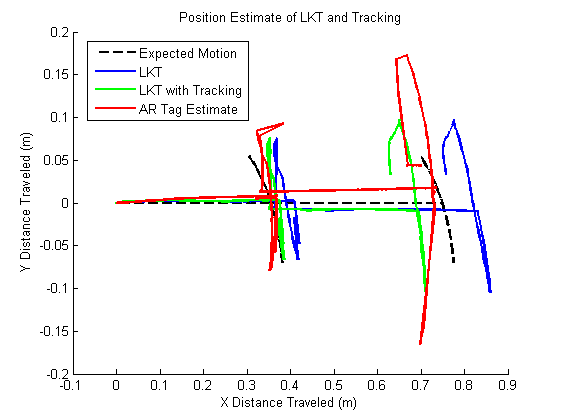
\includegraphics[width=\columnwidth]{crawler1_path.png}
%		  \subcaption{Paths produced by different motion estimates for a simple groundtruth motion.}
%		  \label{crawler:pattern1_path}
%	\end{subfigure}
%	\begin{subfigure}{\columnwidth}
%		  \centering
%		  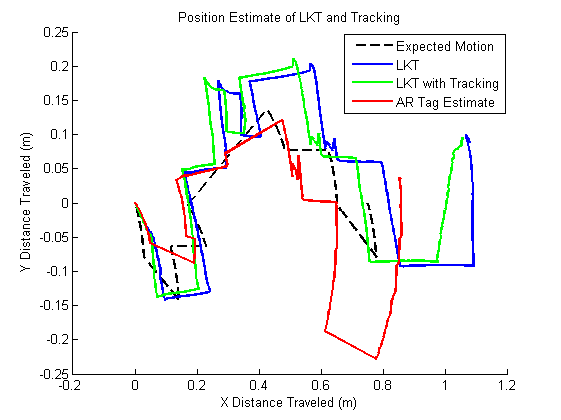
\includegraphics[width=\columnwidth]{crawler2_path.png}
%		  \subcaption{Paths produced by different motion estimates for a more complex groundtruth motion.}
%		  \label{crawler:pattern2_path}
%	\end{subfigure}
%	\caption{Odometry paths generated for multiple motions using the crawler robot.}
%    \label{crawler_path}
%\end{figure*}
%
%\begin{figure*}[tb]
%	\centering
%	\begin{subfigure}{\columnwidth}
%		  \centering
%		  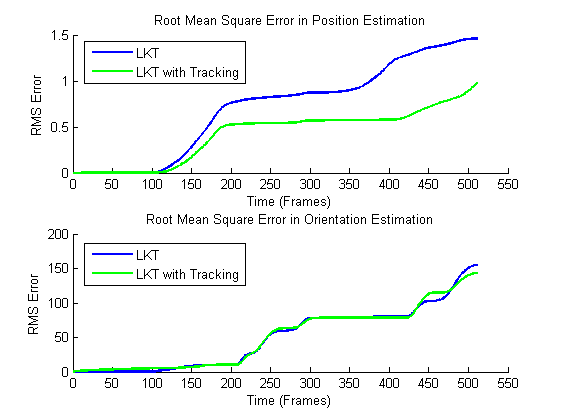
\includegraphics[width=\columnwidth]{crawler1_rms.png}
%		  \subcaption{Error between algorithms and a simple groundtruth motion.}
%		  \label{crawler:pattern1_error}
%	\end{subfigure}
%	\begin{subfigure}{\columnwidth}
%		  \centering
%		  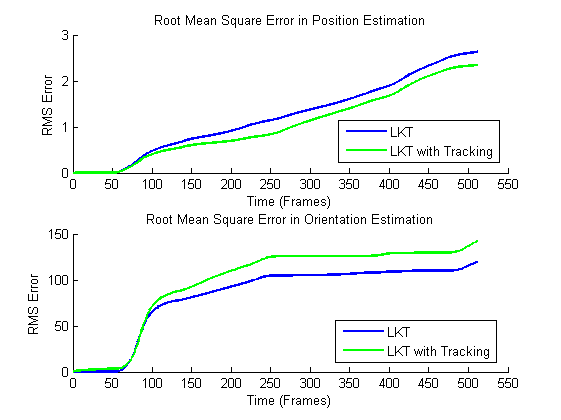
\includegraphics[width=\columnwidth]{crawler2_rms.png}
%		  \subcaption{Error between algorithms and a more complex groundtruth motion.}
%		  \label{crawler:pattern2_error}
%	\end{subfigure}
%	\caption{Comparison of errors between algorithms for multiple motions using the crawler robot.}
%    \label{crawler_error}
%\end{figure*}
%
%\begin{table*}[tb]
%	\centering
%	\footnotesize
%	\setlength{\tabcolsep}{.6em}
%	\caption{Error Statistics for multiple motions with the Crawler Robot}
%	\label{table:crawler_results}
%	\begin{tabular}{c|c|c|c|c|}
%	\hline
%	& Motion 1 & Motion 1 & Motion 2 & Motion 2\\
%	\hline
%	Algorithm & LKT & LKT + Object Tracking & LKT & LKT + Object Tracking\\ 
%	\hline
%	Sum of Squared Position Error & 2.1370 & 0.9534 & 36.453 & 22.263\\
%	\hline
%	Standard Deviation of Squared Position Error & 0.0049 & 0.0031 & 0.034 & 0.025\\
%	\hline
%	Mean Orientation Error & 4.1598 & 3.6811 & 5.3688 & 4.604\\
%	\hline
%	Standard Deviation of Orientation Error & 5.4483 & 5.1506 & 3.9943 & 3.6791\\
%	\hline
%	\end{tabular}
%\end{table*}
%
%\section{Conclusion}
%
%We have proposed a vision system for robots in inspection environments that improves the Lucas-Kanade algorithm by adding a Hough Transform based salient object tracker. In general, Lucas-Kanade provides a starting estimate of the robot's motion by matching the textural components of the image. However, errors in motion estimation accumulate and cause drift. The salient object tracker is more precise for certain components of the robot's motion and is more insensitive to drift, since the tracker senses the same object repeatedly. We have demonstrated incorporating the salient object tracker on multiple inspection robots and shown that it improves Lucas-Kanade for all platforms.



% This command serves to balance the column lengths
% on the last page of the document manually. It shortens
% the textheight of the last page by a suitable amount.
% This command does not take effect until the next page
% so it should come on the page before the last. Make
% sure that you do not shorten the textheight too much.
\addtolength{\textheight}{-1cm}

\section*{Acknowledgment}

The authors would like to thank the current and past members of the Biorobotics Lab for instrumental contributions to the research.

\bibliographystyle{IEEEtran}
\bibliography{IEEEabrv,visual_odometry_paper}

\end{document}